\documentclass{../template/Report}%方括号内写yuxi即生成预习报告\documentclass[yuxi]{../template/Report}
\settemplatedir{../template/}%设置模板路径

\exname{\small 交流电路功率因数实验、组装整流器} %实验名称
\extable{} %实验桌号
\instructor{} %指导教师
\class{} %班级
\name{} %姓名
\stuid{} %学号

\nyear{2025} %年
\nmonth{12} %月
\nday{17} %日
\nweekday{三} %星期几，e.g. \nweekday{三}
\daypart{上午}%上午/下午

\redate{} %如有实验补做，补做日期
\resitu{} %情况说明：
\newcommand{\drawspace}[2]{
    \begin{center}
        \fbox{
            \begin{minipage}{0.9\textwidth}
                \vspace{#1}
                \centering
                \textbf{\textsf{[此处手绘：#2]}}
                \vspace{#1}
            \end{minipage}
        }
    \end{center}
}
\begin{document}
\maketitle%输出封面

\section{预习报告（10分）}
（注：将已经写好的“物理实验预习报告”内容拷贝过来）

\subsection{实验综述（5分）}
（自述实验现象、实验原理和实验方法，包括必要的光路图、电路图、公式等。不超过500字。）

\subsubsection{交流电路功率因数实验}

\paragraph{实验目的与现象}
本实验通过测量交流电路中的功率因数，旨在理解功率因数的物理意义、掌握提高电感性电路功率因数的方法、熟悉日光灯的工作原理。

\paragraph{实验原理}
功率因数为电压与电流相位差的余弦（$\cos\varphi$）。日光灯支路为感性负载，电流滞后于电压，导致功率因数较低。

改善方法：在电路中并联电容器。利用电容电流超前电压的特性，抵消部分感性无功电流，使总电流减小，从而提高功率因数。

\paragraph{实验公式}
\begin{enumerate}
    \item \textbf{有功功率：} $P = UI \cos\varphi$
    \item \textbf{感抗：} $X_L = \frac{U}{I} \sin\varphi$
    \item \textbf{容抗：} $X_C = \frac{1}{\omega C}$
\end{enumerate}

\paragraph{实验电路}
如\cref{fig:不同负载}为包含不同负载的交流电路，通过测量电压、电流和相位差，可以计算出功率因数。
\begin{figure}[H]
    \centering
    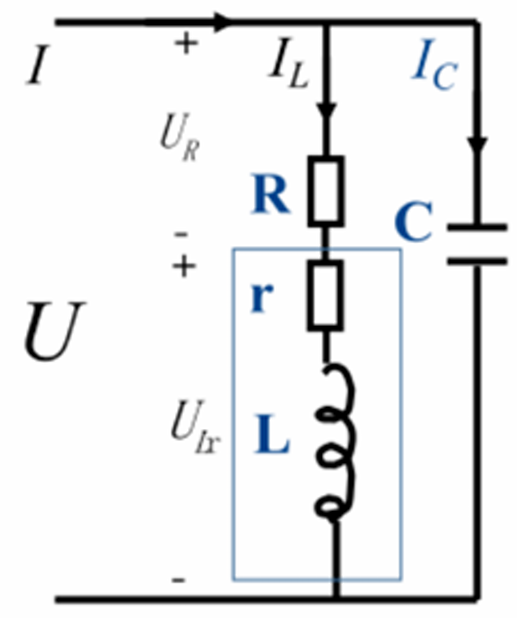
\includegraphics[width=.3\textwidth]{./figures/2/不同负载的交流电路示意图.png}
    \caption{不同负载的交流电路示意图}
    \label{fig:不同负载}
\end{figure}

%-----------------------------------------------------------
\subsubsection{组装整流器}

\paragraph{实验目的}
深入理解整流与滤波电路的功能，掌握单相半波、全波、桥式整流电路及RC滤波电路的设计与组装，探究其输出电压特性。

\paragraph{整流电路分类与特性}

\begin{enumerate}
    \item \textbf{单相半波整流：}
          \begin{itemize}
              \item 利用二极管单向导电性，仅正半周通过。
              \item 输出电压平均值：$\overline{U_0} \approx 0.45 U_2$
          \end{itemize}
          \begin{figure}[H]
              \centering
              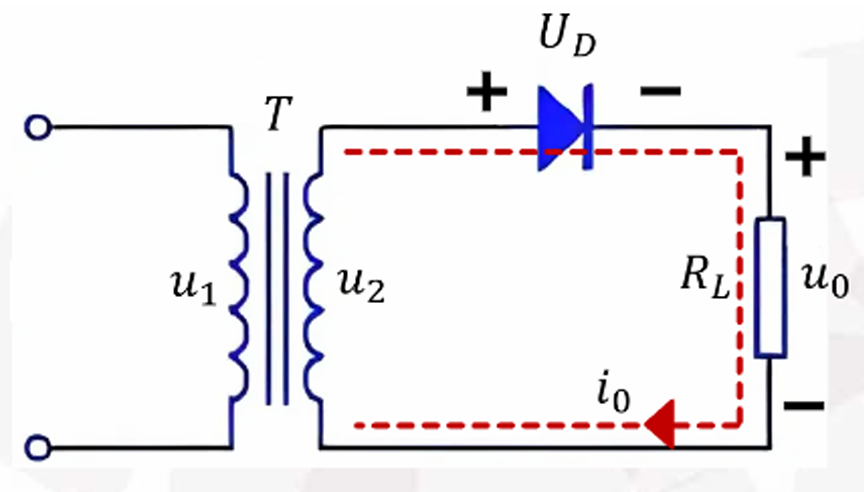
\includegraphics[width=.6\textwidth]{./figures/2/单相半波整流电路.png}
              \caption{单相半波整流电路}
          \end{figure}

    \item \textbf{单相全波整流：}
          \begin{itemize}
              \item 需带中心抽头的变压器，正负半周均利用。
              \item 输出电压平均值：$\overline{U_0} \approx 0.9 U_2$
              \item 二极管承受最大反向电压较高：$U_{Dmax} = 2\sqrt{2}U_2$
          \end{itemize}
          \begin{figure}[H]
              \centering
              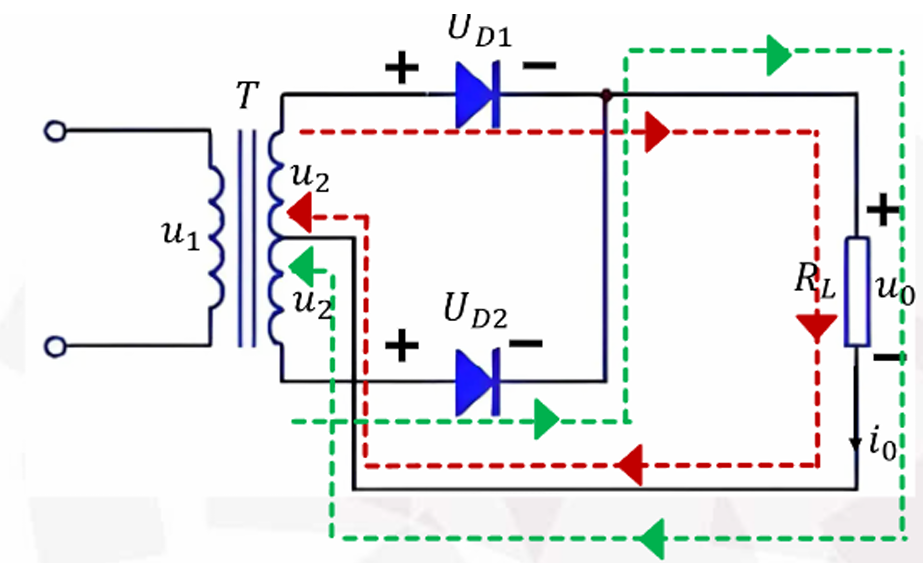
\includegraphics[width=.6\textwidth]{./figures/2/单相全波整流电路.png}
              \caption{单相全波整流电路}
          \end{figure}

    \item \textbf{单相桥式整流：}
          \begin{itemize}
              \item 由四个二极管组成桥路，无需中心抽头即可利用正负半周。
              \item 输出电压平均值：$\overline{U_0} \approx 0.9 U_2$
              \item 二极管承受最大反向电压：$U_{Dmax} = \sqrt{2}U_2$
          \end{itemize}
          \begin{figure}[H]
              \centering
              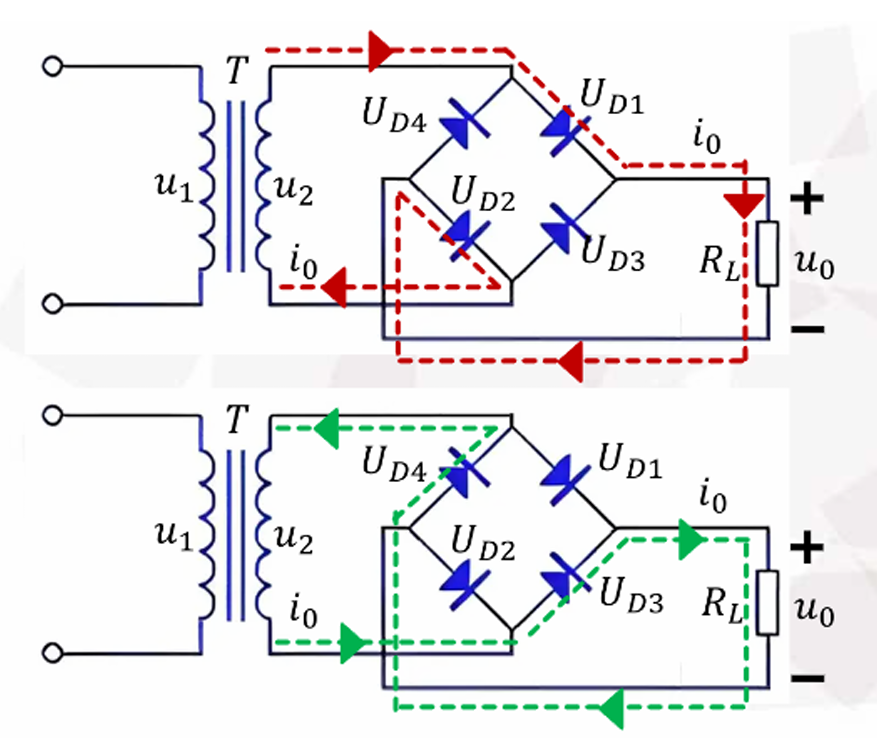
\includegraphics[width=.6\textwidth]{./figures/2/单相桥式整流.png}
              \caption{单相桥式整流电路}
          \end{figure}
\end{enumerate}

\paragraph{滤波电路}
利用电容的充放电特性滤除交流分量。电容充电时存储电能，放电时释放电能，使输出电压更平滑。
\begin{figure}[H]
    \centering
    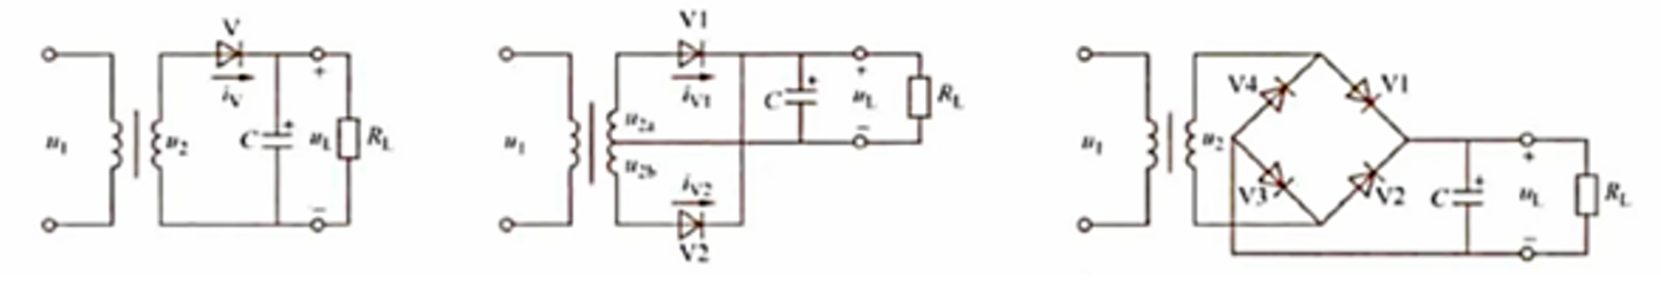
\includegraphics[width=.6\textwidth]{./figures/2/RC滤波.png}
    \caption{RC滤波电路}
\end{figure}

\subsection{实验重点（3分）}
（简述本实验的学习重点，不超过100字。）

\begin{enumerate}
    \item \textbf{功率因数实验：} 理解功率因数的定义($\cos \varphi = \frac{P}{UI}$)及其物理意义，掌握感性负载功率因数的测量及通过并联电容提高功率因数的方法。
    \item \textbf{整流器组装：} 掌握半波、全波、桥式整流及RC滤波的原理与核心公式，学会使用示波器观测波形并测量参数。
\end{enumerate}

\subsection{实验难点（2分）}
（简述本实验的实现难点，不超过100字。）

\begin{enumerate}
    \item \textbf{数据规律：} 需精准测量不同电容下的电参数，准确分析功率因数随电容变化的非单调（先升后降）规律。
    \item \textbf{电路搭建：} 整流电路搭建较复杂，二极管极性及电解电容极性易接反，需仔细检查。
\end{enumerate}

\begin{fullreportonly}
    \section{原始数据（20分）}
    % 这里通常需要插入您那两张原始数据纸张的照片
    \begin{figure}[H]
        \centering
        % \includegraphics[width=0.8\textwidth]{original_data_scan.jpg}
        \caption{原始数据记录表}
    \end{figure}

    \section{结果与分析（60分）}

    \subsection{数据处理与结果（30分）}

    \subsubsection{交流电功率因数}

    根据实验测量数据，计算功率因数 $\cos\varphi = \frac{P}{U \cdot I}$，结果如下表所示：

    \begin{table}[H]
        \centering
        \caption{交流电功率因数测量数据表}
        \begin{tabular}{|c|c|c|c|c|}
            \hline
            电容 $C$ (\unit{\micro\farad}) & 电压 $U$ (\unit{\volt}) & 电流 $I$ (\unit{\milli\ampere}) & 功率 $P$ (\unit{\watt}) & 功率因数 $\cos\varphi$ \\ \hline
            1                            & 223.6                 & 258.3                         & 23.5                  & 0.407              \\ \hline
            2                            & 223.6                 & 200.8                         & 23.2                  & 0.517              \\ \hline
            3                            & 223.8                 & 159.0                         & 23.4                  & 0.658              \\ \hline
            4                            & 224.0                 & 126.0                         & 23.8                  & 0.843              \\ \hline
            5                            & 224.1                 & 126.9                         & 23.7                  & 0.833              \\ \hline
            6                            & 223.9                 & 159.3                         & 24.3                  & 0.681              \\ \hline
            7                            & 224.0                 & 201.4                         & 24.5                  & 0.543              \\ \hline
            8                            & 224.2                 & 242.4                         & 24.1                  & 0.443              \\ \hline
            9                            & 224.1                 & 299.2                         & 25.0                  & 0.373              \\ \hline
        \end{tabular}
    \end{table}

    \textbf{图像分析：}
    利用MATLAB绘制功率因数 $\cos\varphi$ 随电容 $C$ 变化的曲线如下图所示。

    \begin{figure}[H]
        \centering
        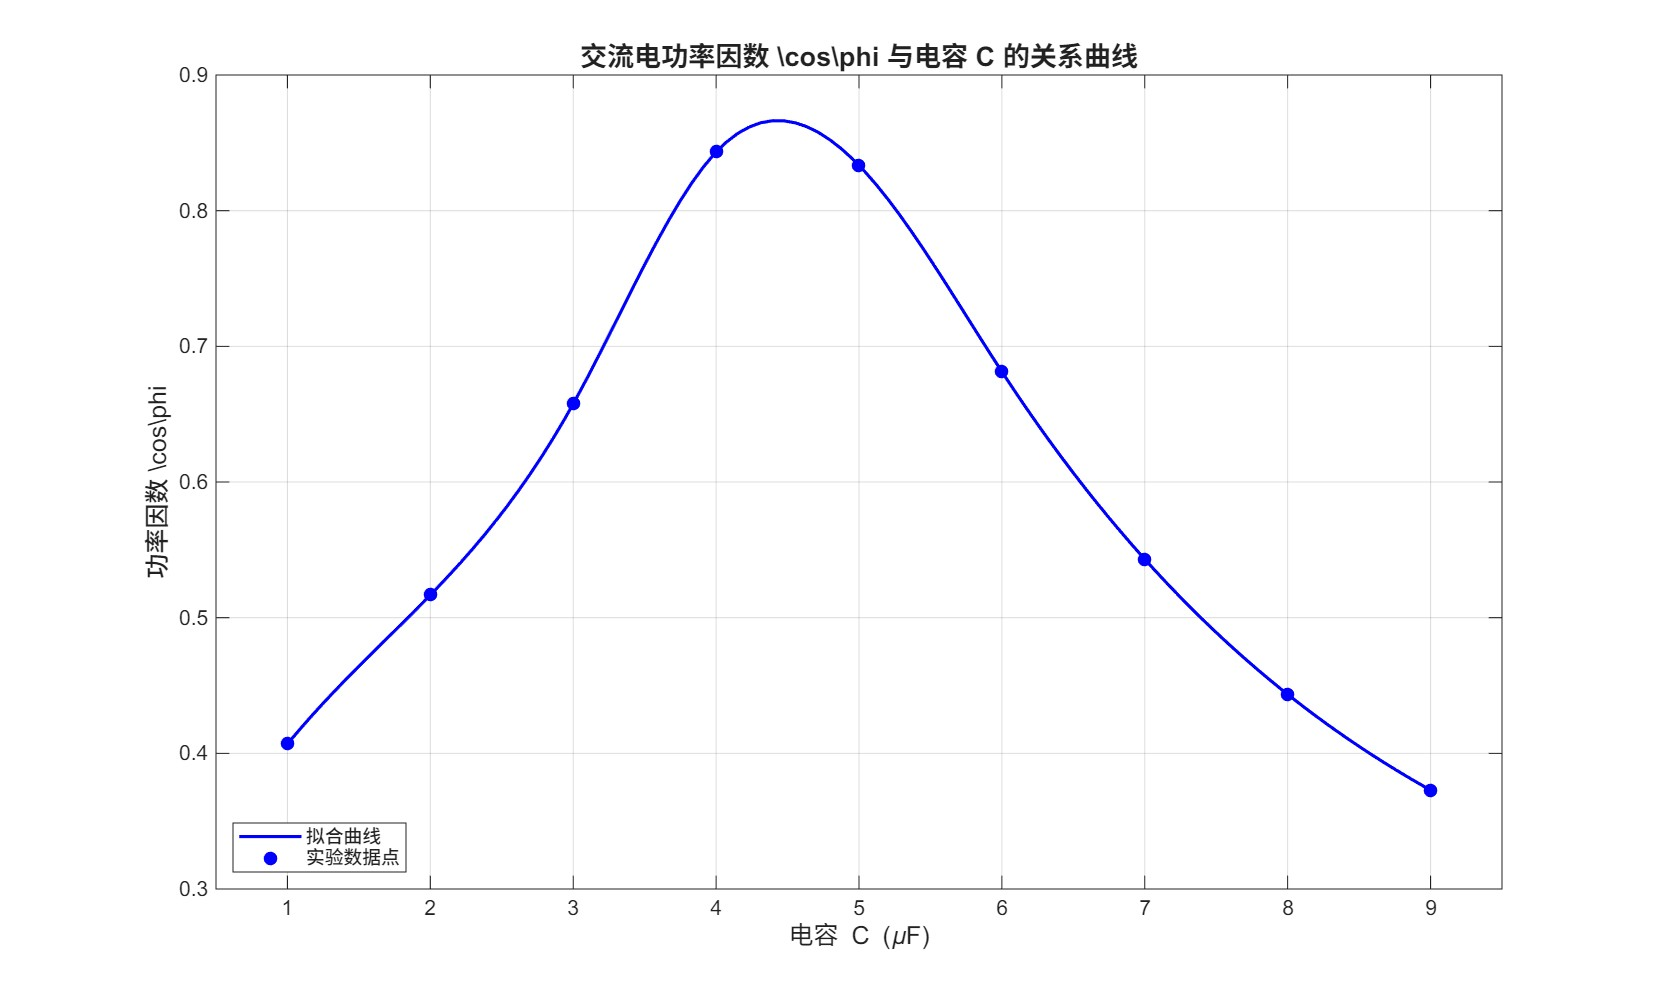
\includegraphics[width=0.75\textwidth]{./figures/2/cos_plot.jpg}
        \caption{功率因数 $\cos\varphi$ 与电容 $C$ 的关系曲线}
    \end{figure}

    \textbf{结论：}
    由数据和图像可知，随着电容值的增加，电路的功率因数先增大后减小。
    \begin{itemize}
        \item 当 $C < \SI{4}{\micro\farad}$ 时，$\cos\varphi$ 随 $C$ 增加而增大；
        \item 当 $C > \SI{5}{\micro\farad}$ 时，$\cos\varphi$ 随 $C$ 增加而减小；
        \item 根据实验记录，在 $C = \SI{5}{\micro\farad}$ 时观察到功率因数较高，
              此时电路处于接近谐振的状态，表现出类似电阻的特性，输入与输出的相位差也比较接近，此时电路的总功率约为 \SI{23.7}{\watt}。
    \end{itemize}

    \subsubsection{组装整流器}

    整流电路的转换系数定义为 $K = \frac{\overline{U_{\text{out}}}}{U_{\text{in\text{有效值}}}}$。其中输入电压有效值由峰峰值换算得到：$U_{\text{in(rms)}} = \frac{U_{\text{p-p}}}{2\sqrt{2}}$。

    \begin{table}[H]
        \centering
        \caption{整流电路数据处理表}
        \begin{tabular}{|c|c|c|c|c|c|}
            \hline
            电路类型 & $U_{\text{p-p}}$ (\unit{\volt}) & $U_{\text{in\text{有效值}}}$ (\unit{\volt}) & $\overline{U_{\text{out}}}$ (\unit{\volt}) & 转换系数 $K$ & 理论 $K$ \\ \hline
            单相半波 & 36.80                           & 12.79                                    & 4.881                                      & 0.382    & 0.45   \\ \hline
            单相全波 & 18.60                           & 6.39                                     & 5.028                                      & 0.787    & 0.90   \\ \hline
            单相桥式 & 36.00                           & 12.45                                    & 9.707                                      & 0.780    & 0.90   \\ \hline
        \end{tabular}
    \end{table}

    \textbf{波形定性描述：}
    \begin{itemize}
        \item  \textbf{半波整流：} 输出波形只保留了正弦波的正半周，负半周被截止，波形间断。
        \item  \textbf{全波整流/桥式整流：} 正负半周均被利用，输出为连续的单向脉动直流电。
    \end{itemize}

    \begin{figure}[H]
        \centering
        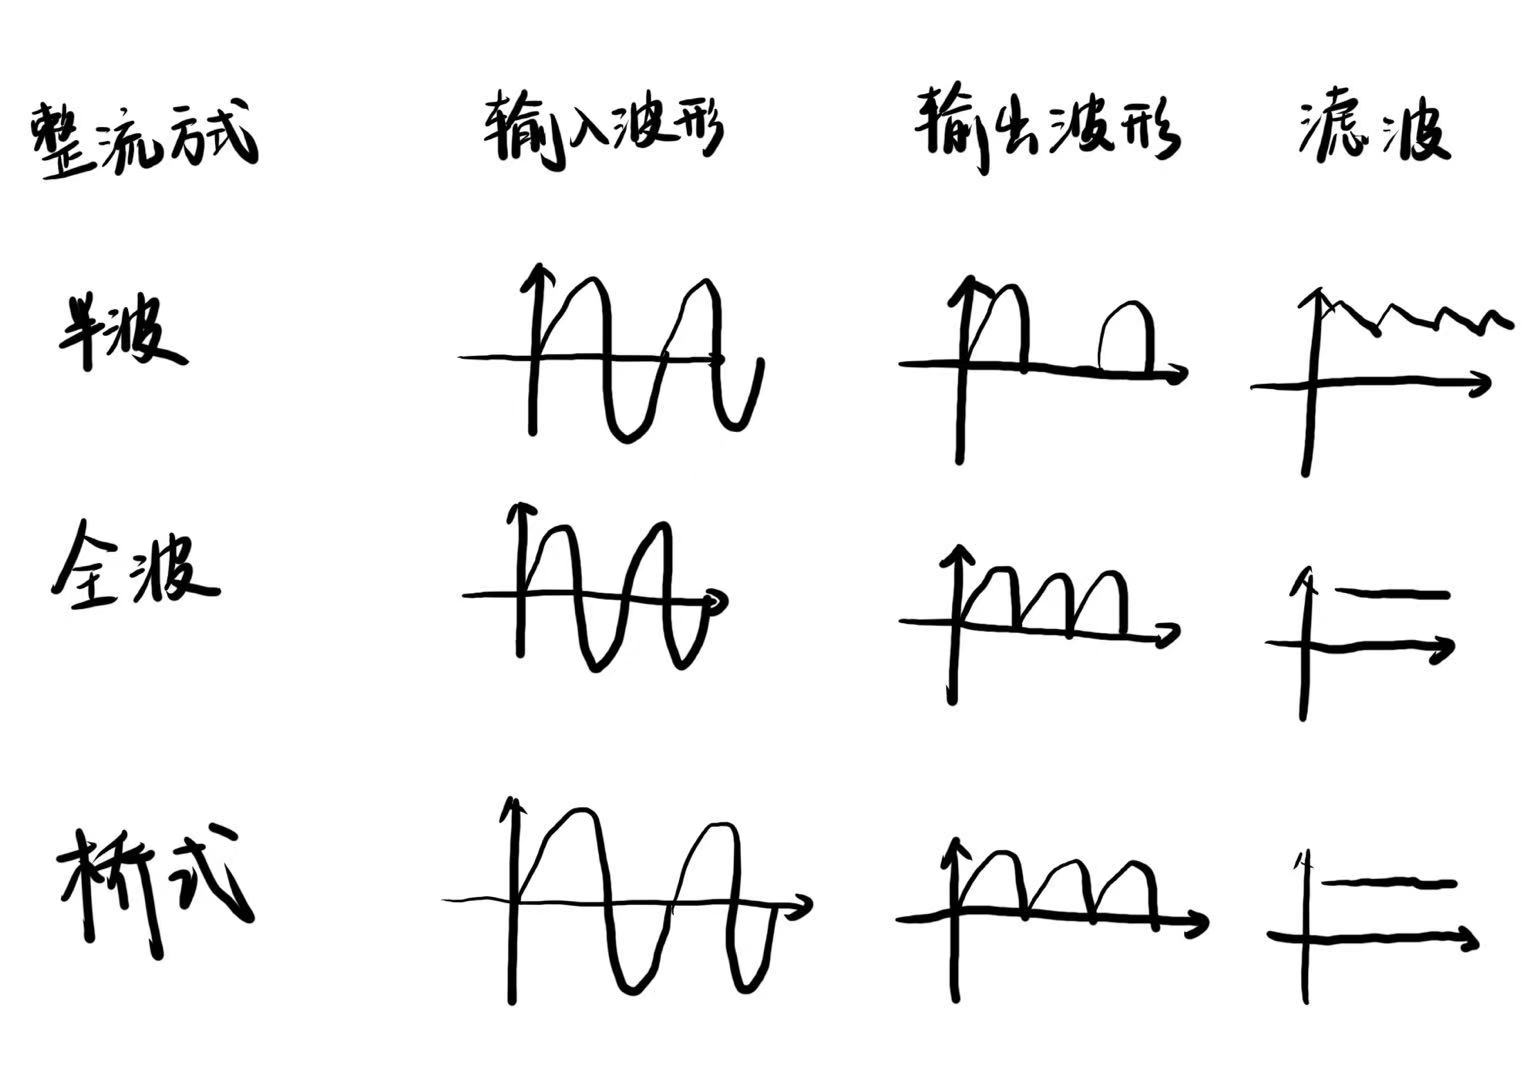
\includegraphics[width=0.75\textwidth]{./figures/2/图像.jpg}
        \caption{不同整流电路的输入输出以及滤波后的波形定性图}
    \end{figure}
    其中由于经过了二极管，单相半波，单相全波整流电路中都会出现压降，而桥式整流经过两个二极管，压降更厉害。

    单相全波整流由于是从变压器的中心抽头取电，所以输入输出电压均较低。

    选取合适的滤波电容后，输出波形从原来馒头型的脉动直流电变成了平滑的直流电，但还是带有略微锯齿。

    \subsection{误差分析（20分）}

    \subsubsection{交流电功率因数}
    \begin{itemize}
        \item 仪表读数误差： 实验中使用的功率表、电压表和电流表存在固有的精度限制，且读数时存在视差。
        \item 元件非理想性： 电感线圈存在内阻，电容存在漏电流，导致实际电路并非理想的RLC模型。
        \item 热效应： 长时间通电导致线圈温度升高，电阻值发生漂移，影响电流和功率的测量。
    \end{itemize}

    \subsubsection{整流器实验误差分析}
    根据实验数据计算，各整流电路转换系数的相对误差如下：
    \begin{itemize}
        \item \textbf{单相半波：} $\eta_1 = \left| \frac{0.382-0.45}{0.45} \right| \times \SI{100}{\percent} \approx \SI{15.1}{\percent}$
        \item \textbf{单相全波：} $\eta_2 = \left| \frac{0.787-0.90}{0.90} \right| \times \SI{100}{\percent} \approx \SI{12.6}{\percent}$
        \item \textbf{单相桥式：} $\eta_3 = \left| \frac{0.780-0.90}{0.90} \right| \times \SI{100}{\percent} \approx \SI{13.3}{\percent}$
    \end{itemize}

    \textbf{误差主要来源分析：}

    实验测得的转换系数 $K$ 均低于理论值（0.45 和 0.90），且误差较大（约 \SI{12}{\percent} 至 \SI{15}{\percent}）。主要原因是理论公式推导时将二极管视为理想开关，忽略了其正向导通压降 $V_D$（硅管约为 \SI{0.7}{\volt}）。由于本次实验输入电压较低（有效值仅约 \SI{6}{\volt} 至 \SI{12}{\volt}），二极管压降占比不可忽略。

    可以通过考虑压降后的理论值来验证数据的合理性：
    \begin{itemize}
        \item \textbf{全波整流验证：} 理论输出电压应为 $U_o \approx 0.9 U_2 - V_D$。
              代入数据计算：$0.9 \times 6.39 - 0.7 = \SI{5.051}{\volt}$。
              该值与实测值 \SI{5.028}{\volt} 非常接近，说明实验数据准确。

        \item \textbf{桥式整流验证：} 电路工作时回路中始终有两个二极管导通，理论输出应为 $U_o \approx 0.9 U_2 - 2V_D$。
              代入数据计算：$0.9 \times 12.45 - 1.4 = \SI{9.805}{\volt}$。
              该值与实测值 \SI{9.707}{\volt} 同样吻合度极高。
    \end{itemize}

    \textbf{结论：} 实验结果虽与理想理论值存在偏差，但若考虑二极管压降修正，实测数据与理论预期高度一致，验证了非理想条件下整流电路的工作特性。

    \subsection{实验探讨（10分）}
    本次实验探究了并联电容对提高电路功率因数的作用。实验表明，适当选择电容值可以显著降低无功功率，减小总电流，提高能源利用率。在整流实验中，验证了不同整流方式的输出特性。桥式整流虽然使用了四个二极管，但无需中心抽头变压器，且对变压器利用率较高。实验中二极管压降对低压整流电路的输出电压有显著影响。

    \section{思考题（10分）}

    \subsection{交流电功率因数}

    \subsubsection{提高功率因数的意义何在？为什么并联电容能提高功率因数？并联的电容是否越大越好？}

    提高功率因数可以节能。在输电过程中，提高 $\cos\phi$ 变压器等发电设备的实际带载能力。

    之所以采用并联电容，是因为实验中大多数负载呈感性，电流滞后于电压。并联电容后，电容支路产生的超前电流恰好能抵消掉负载所需的滞后无功电流。这样一来，电源只需要提供有功分量，总电流就减小了。

    不过，并联电容并非越大越好。当补偿刚好使得电路呈纯电阻性时，效果最佳。如果继续增大电容，电路会由感性转变为容性。此时容性无功电流占据主导，总电流反而会重新增大，甚至可能引起线路电压异常升高，造成电流损失。

    \subsubsection{在实验中，随着电容增加，电路总电流的变化规律为由大变小再变大，试分析原因。}

    这个现象可以用电流矢量的合成来解释。实验初始阶段，负载是感性的，总电流中包含较大的感性无功分量。随着并联电容 $C$ 的增加，它产生的容性电流与感性电流方向相反，这些电流开始抵消感性分量，使得总电流的矢量模长逐渐减小。

    当电容增加到谐振点时，感性电流和容性电流基本相互抵消，电路接近纯电阻状态，此时总电流达到最小值。一旦跨过这个点继续增加电容，容性电流就会超过感性电流，电路性质转变为容性。随着电容进一步增大，过剩的容性电流使得总电流再次开始上升。

    这就是电流呈现先变小再变大的原因。

    \subsubsection{在进行功率因数补偿时，本实验采用并联电容器的方法，为什么不采用串联电容器的方法？}

    首先是电压稳定性的考虑。负载通常需要稳定的额定电压才能正常工作。并联电容器不改变负载两端的电压；而如果串联电容，电容会有分压作用，导致负载两端的电压随电流变化而波动，设备无法正常工作。

    其次是安全问题。串联电容和电感很容易构成串联谐振电路。在谐振状态下，电感和电容两端可能会产生数倍于电源电压的高压，这极易击穿电容器绝缘层或烧毁负载，引发安全事故。

    \subsection{组装整流器}

    \subsubsection{总结不同的整流电路和不同的滤波电路的利弊？}

    对于整流电路：\textbf{单相半波}结构最简单，只要一个二极管，但它浪费了半个周期的波形，效率低且纹波大，只适合要求极低的小功率场合；\textbf{全波整流}虽然效率高，但必须配合带中心抽头的变压器，这增加了变压器的体积和制作难度；\textbf{桥式整流}是目前最通用的方案，它不需要中心抽头，对变压器要求低，输出纹波小，唯一的代价是多用了两个二极管，但这在现代电路中成本几乎可以忽略。

    对于滤波电路：\textbf{电容滤波}最简单经济，适合负载电流较小的情况，但其输出电压受负载电阻影响大；而\textbf{LC滤波}虽然波形更平滑且带载能力强，但电感体积大且笨重，现在一般只在特定的大功率或高频电源中使用。

    \subsubsection{整流和滤波的目的是什么？}

    整流利用二极管的单向导电性，把正负交替变化的交流电变成方向单一、但大小还在跳动的脉动直流电。

    滤波利用电容两端电压不能突变的特性，把脉动直流电中波动的交流分量滤掉，让输出电压尽量平滑，类似实验室常用的恒稳直流电源。

    \subsubsection{如何根据需要选择合适的整流电路？}

    选择电路主要看具体的应用需求。
    如果是给普通的电子设备供电，桥式整流通常是首选，因为其综合性能最好，变压器利用率高。如果受限于变压器参数（比如已经有了中心抽头变压器），或者是在极低电压下工作，可以选择全波整流。

    而在一些对波形要求极低、仅仅是需要把电热丝加热或者简单的信号检测电路中，为了省成本和空间，才会考虑使用半波整流。
\insertnotes
\end{document}